\section{Analyse}

\subsection{Problemraum und Anforderungen}
Für den Empfang von Messdaten und die korrekte Startvorbereitung benötigen Radiosonden von GRAW auch immer eine Bodenstation.
Auf Bodenstationen läuft unter Windows die Software \enquote{GRAWMET}\cite{grawmet}, welche die Messdaten der Sonde empfängt, weiterverarbeitet und auswertet.
Um vergangene Flüge auszuwerten und zu überwachen, ist daher immer der Zugang zum Bodenstationscomputer notwendig.
Eine zentrale und einfache Auswertung mehrerer Stationen, durch Nutzer an verschiedenen Orten, mit verschiedenen Endgeräten, ist aktuell kaum möglich.
Es gibt für diese Anforderungen bereits eine experimentelle Anwendung \enquote{GRAWgo}\cite{grawgo}, welche aufgrund ihrer Architektur kein On-Premises Hosting unterstützt und nur auf Mobilgeräten lauffähig ist.
GRAWgo ist mit seiner sehr eingeschränkten Nutzbarkeit bisher nicht für den produktiven Betrieb im Bereich größerer Messnetze konzipiert und wird hier in der Folge nicht eingesetzt

Diese Problemstellung soll durch eine neue Architektur, bzw.\ eine ergänzende Software namens \enquote{Sounding Console}, gelöst werden.
Der Zugang, zu den erfassten Daten und Auswertungen, soll vereinfacht werden und von verschiedenen Orten aus möglich sein.
Hier setzt die Sounding Console an und soll die daraus resultierenden Anforderungen erfüllen.

Grundsätzlich wurden durch den Auftraggeber Anforderungen im Rahmen eines Lastenheftes (\ref{subsec:lastenheft}) kommuniziert.
Diese wurden durch den Verfasser dieser Arbeit zunächst technisch eingeordnet und, soweit für die Auftragsklärung erforderlich, in Teilen angepasst und ergänzt.
Auf dieser Basis wurde durch die auftragnehmende Agentur ein Angebot (\ref{subsec:angebot}) erstellt.
Nach Auftragseingang wurden die konkreteren Anforderungen und daraus resultierende Aufgaben durch den Entwickler im sogenannten Leistungspaket (\ref{subsec:leistungspaket}) detailliert festgelegt.
Offene Fragen wurden in diesem Schritt direkt mit dem Auftraggeber geklärt.

Im Folgenden sind die Anforderungen aufgeführt, die die neue Software erfüllen soll.
Die detaillierte Darstellung findet sich im Anhang dieser Arbeit.

\newpage

\subsubsection{Inhaltliche Anforderungen}
Die im folgenden gelisteten inhaltlichen Anforderungen wurden überwiegend seitens des Auftraggebers erarbeitet, ergaben sich aber auch in Teilen aus konkreten Rückfragen im Entwicklungsprozess.
\begin{itemize}
    \item Administratoren müssen Nutzern den Zugriff auf die Software ermöglichen können und diesen durch eine Rollenzuweisung mit unterschiedlichen Zugriffsrechten einschränken können.
    \item Im System müssen mehrere Bodenstationen verwaltet werden können.\ Deren Sichtbarkeit muss auf spezifische Nutzer eingeschränkt werden können.
    \item Die Flugdaten der Radiosonden müssen via Schnittstelle, von mehreren Bodenstationen gleichzeitig, empfangen werden können.
    \item Die Kommunikation mit den Stationen soll nahezu in Echtzeit funktionieren.
    \item Es sollen Flüge und deren Messdaten aus bestehenden Archiven importiert werden können.
    \item Eine sprachliche Internationalisierung muss möglich sein.
    \item Je Flug müssen eindimensionale Performancekriterien berechnet und angezeigt werden können.
    \item Die Performance einer Station soll, mittels durchschnittlicher Performancekriterien aus vergangenen Flügen, in unterschiedlichen Zeitabschnitten einsehbar sein.
    \item Flugdaten sollen in Echtzeit verfolgt werden können und müssen im Nachhinein auswertbar sein.
    \item Es soll eine Kartendarstellung von einem oder mehreren Flügen geben.\ Dafür soll der Einsatz eines Open Source Projektes\cite{sondehub-tracker} geprüft werden.
    \item Für einen Flug müssen Messdaten tabellarisch dargestellt werden können.
    \item Je Flug müssen einige Messdaten in zweidimensionalen Liniendiagrammen gegenüber Zeit, Höhe und Luftdruck dargestellt werden können.
    \item Es soll geprüft werden, ob mit überschaubarem Aufwand auch thermodynamische Diagramme dargestellt werden können.
\end{itemize}
\newpage

\subsubsection{Technische Anforderungen}
Die technische Anforderungen wurden von beiden Parteien gemeinsam festgelegt.
Dabei wurden die vorhandenen Kompetenzen und Erfahrungswerte hinsichtlich Programmiersprachen und Frameworks seitens des Entwicklers berücksichtigt.
Einige Entscheidungen berücksichtigen zudem, dass die Entwicklung mit möglichst geringen finanziellen Ressourcen erfolgen kann.
\begin{itemize}
    \item Die Software muss auf einer zentralen Instanz gehostet werden. Dies muss sowohl auf zentralen Servern als auch On-Premises möglich sein.
    \begin{itemize}
        \item Es sollen aktuelle Standards wie Docker und Kubernetes verwendet werden.
    \end{itemize}
    \item Die Sounding Console soll gegenüber GRAWgo eine verbesserte Zugänglichkeit und UX aufweisen, insbesondere die Nutzung an einem Desktop Computer soll ermöglicht werden.
    \begin{itemize}
        \item Das System soll webbasiert umgesetzt und deployed werden.
        \item Das Interface soll responsive auf verschiedene Bildschirmgrößen reagieren.
    \end{itemize}
    \item Die Software soll durch die Verwendung moderner, bekannter, sowie quelloffener Frameworks entwickelt werden.
    \item Durch die Verwendung von Industriestandards soll eine externe Abhängigkeit gegenüber dem Auftragnehmer verhindert werden.
    \item Die sprachliche Internationalisierung soll, durch die Erstellung und Einbindung neuer Sprachdateien, effizient möglich sein.
    \item Das Projekt muss mittels git versioniert werden.
    \item Automatische Deployments sollen schnelle Updates der Test- und Produktivumgebung ermöglichen.
\end{itemize}

\subsection{Themenfeldanalyse}
Die folgende visuelle Analyse (\ref{fig:themenfeldanalyse}) gibt einen besseren Überblick über das Themenfeld, welches sich aus der zentralen Projektfrage ableiten lässt.
Außerdem werden übliche, grundsätzlich geeignete technische Frameworks betrachtet, die im Projektverlauf von Vorteil sind.

\newpage
\begin{figure}[h!]
    \centering
    \caption{Themenfeldanalyse}
    \label{fig:themenfeldanalyse}
    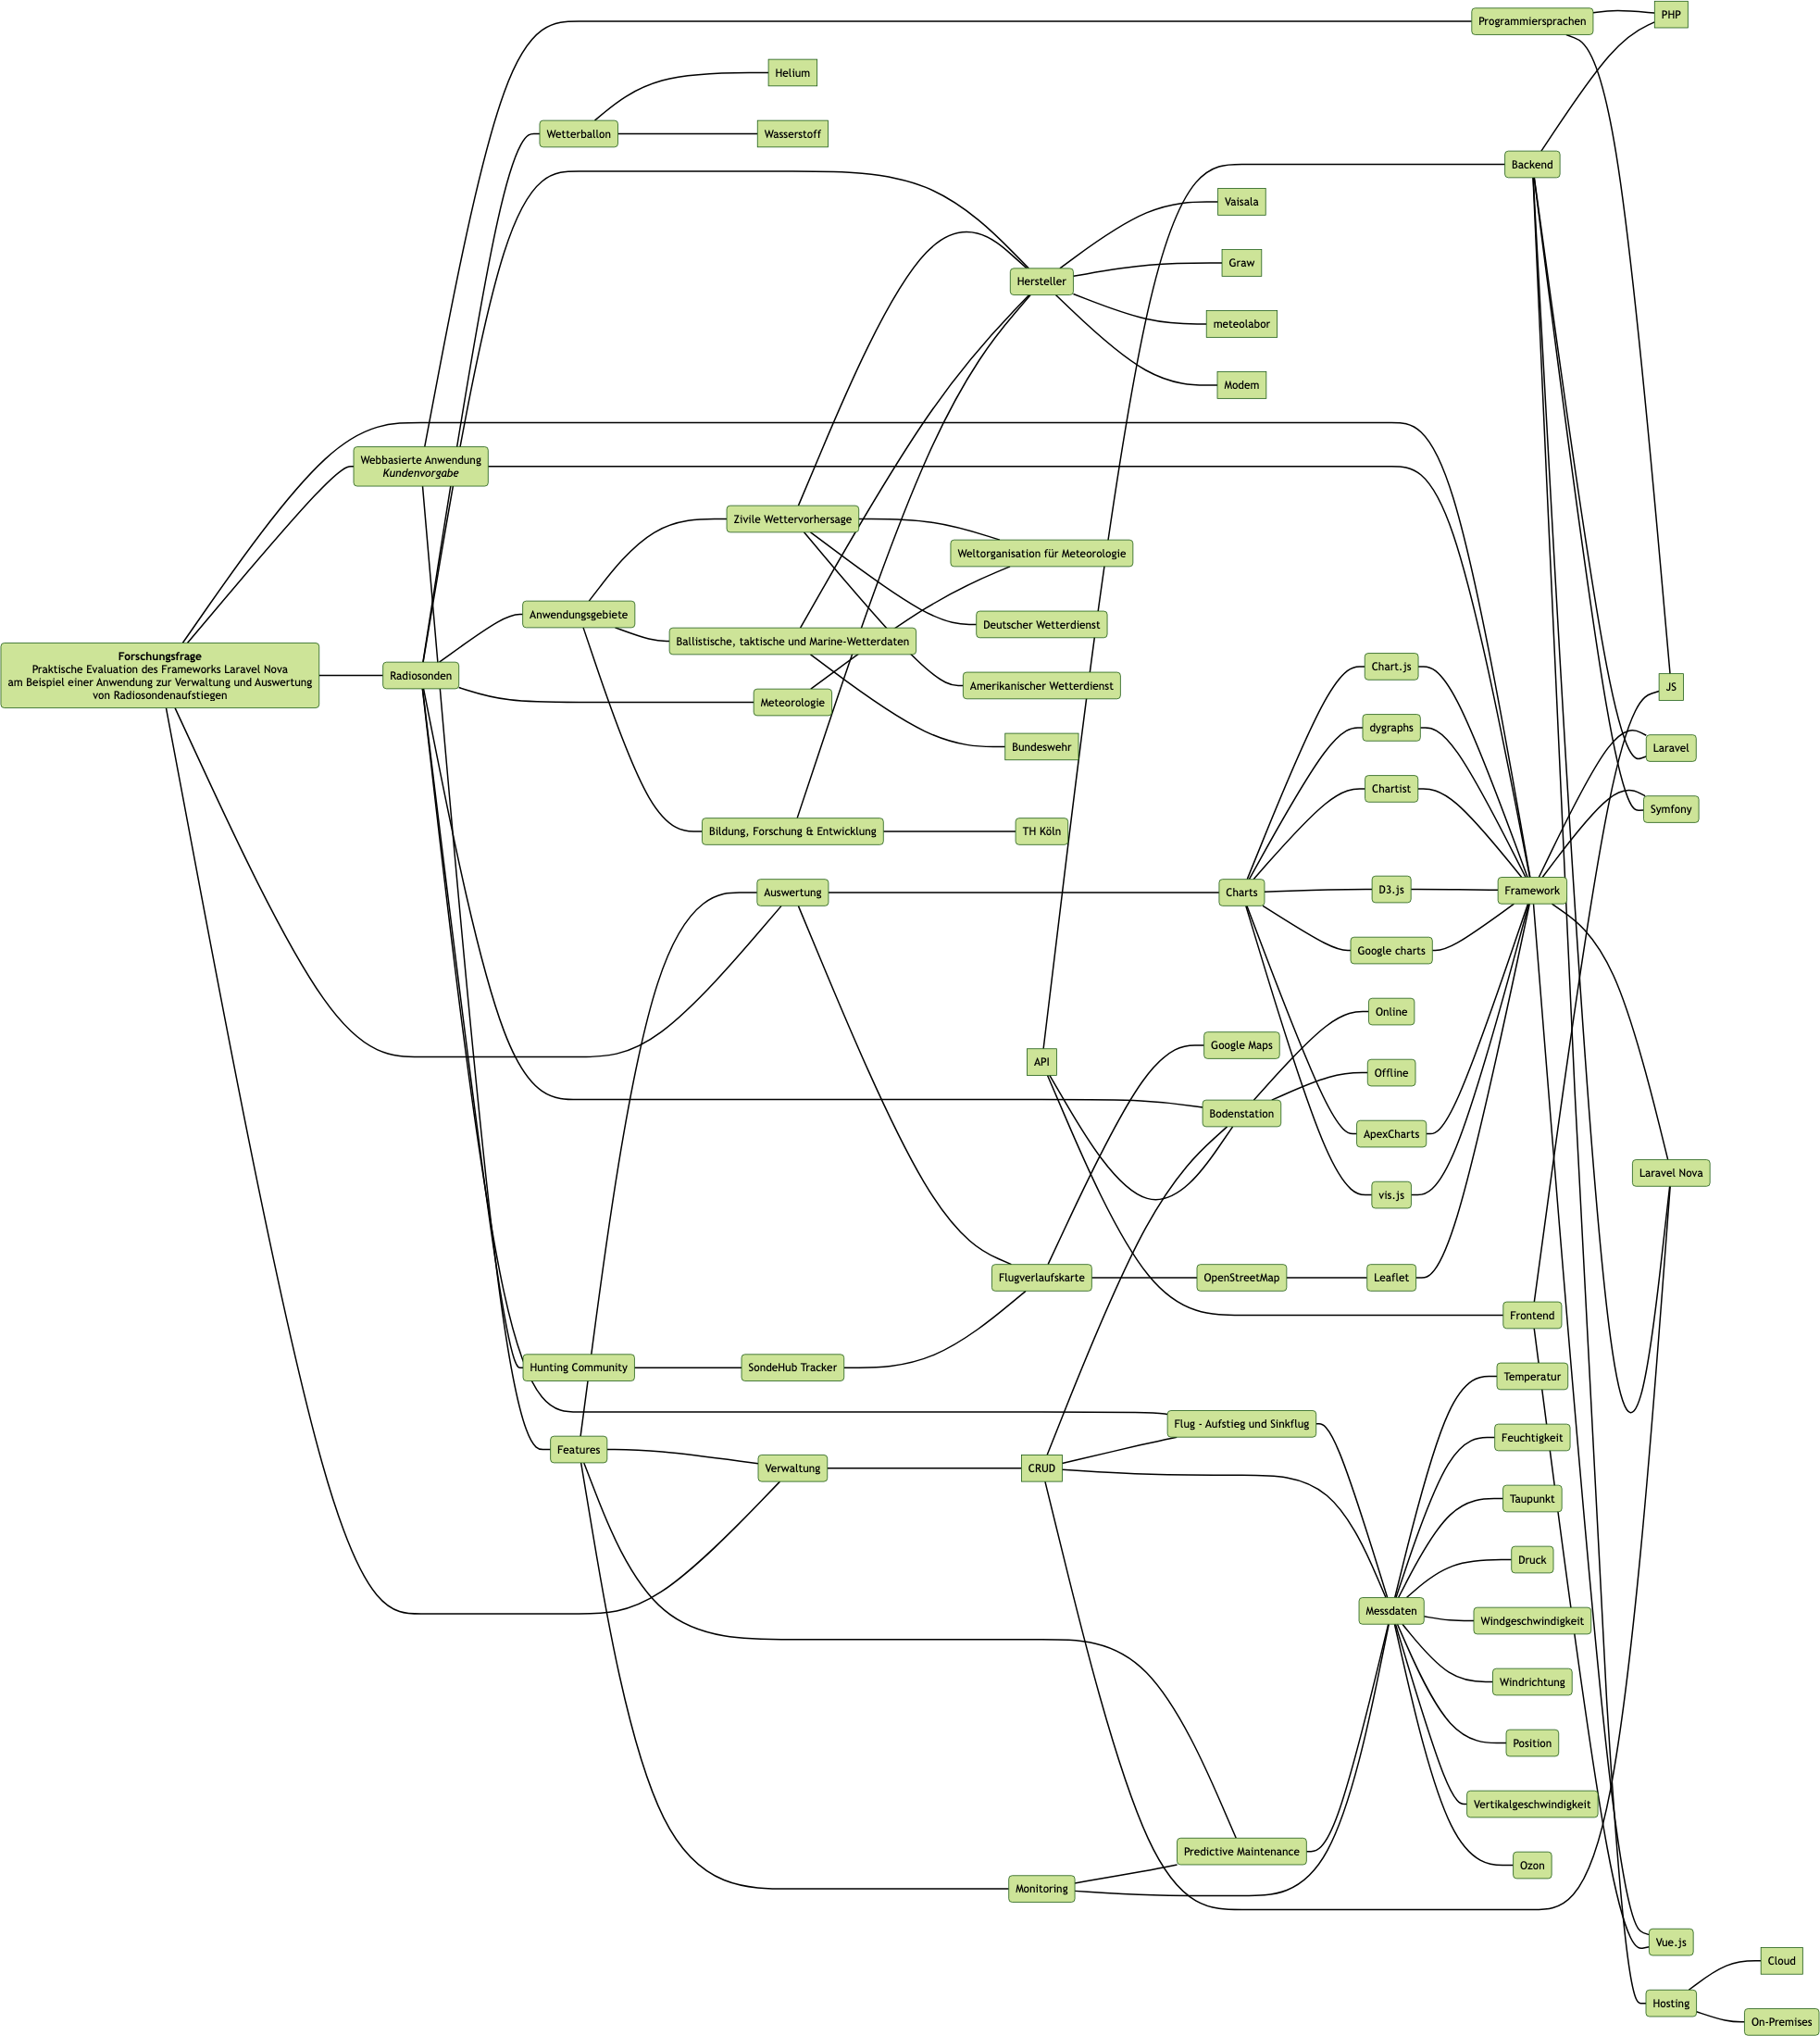
\includegraphics[scale=0.255]{assets/themenfeldanalyse_no_padding}
\end{figure}
\newpage
